\chapter{Timing}
\section{What is timing .:}
    
    % Colocar definição do aprendizado de reforço
    Mechanisms for measuring time are found in a variety of organisms, from humans to plants \cite{cashmore2003cryptochromes}. Initially bound by external rhythms (like circadian cycles), time estimation mechanisms were among the first competencies evolved in biological systems \cite{paranjpe2005evolution}, and are constitutive of many other cognitive modalities such as decision making and episodic memory \cite{maniadakis2014time}. Most behavior is inseparable from a temporal or rhythmic component \cite{buhusi2005makes}. From deciding to accelerate or break in a yellow light, through the simple motor organization of walking or running, to the complex dynamics of speech and musical performance, computational processes are temporally structured to correct execution \cite{bueti2014temporal}. 
    
    While organisms and their brains have to account for event durations in many timescales, from milliseconds to days, there is no single neural correlate able to account for them all \cite{buhusi2005makes, buhusi2016clocks, hardy2016neurocomputational, lewis2003distinct, mauk2004neural}. On the one hand, circadian rhythms depend on the suprachiasmatic nucleus (SCN), relying on slow protein cycles managed by transcriptional feedback loops \cite{buhusi2005makes}, and are important to regulate social and foraging behavior. In turn, the temporal structure of milliseconds relies on local circuits and their communication with the cerebellum \cite{ohmae2017cerebellar}, and is essential to fine motor control, such as playing an instrument or making a tool. In between, the time scale of seconds is central to planning, decision making and reasoning \cite{buhusi2005makes}, and is dependent on the Striatum \cite{mello2015scalable}, but independent of the SCN \cite{lewis2003interval}, and cerebellum \cite{harrington2004does}. The present work focuses in the scale of seconds, named as \textit{interval timing}.
    
    The scale of seconds is less well-understood than its counterparts, but there is much experimental evidence about regions and mechanisms involved in its estimation. Evidence comes from a variety of sources, from psychophysics \cite{ohmae2017cerebellar} and pharmacology \cite{pine2010dopamine, meck2012gene, drew2003effects, cheng2016clock, ludvig2008stimulus} to lesion studies \cite{} and electrophysiology \cite{bakhurin2017differential}. From psychophysics, we know that time estimation obeys Weber's law \cite{gibbon1977scalar}, meaning that the error is proportional to the mean, and thus time-scale invariant; From pharmacology, we know that dopamine agonists shorten time estimates while antagonists elongate them \cite{}; Lesion studies show some regions necessary for timing behavior \cite{};
    Lastly, electrophysiology shows neural correlates of timing \cite{}.
    
    % In the rest of this chapter we will present two complementary ways of characterizing
    
\section{Timing models}
\label{sec:models}
    The Scalar Expectancy Theory (SET) proposes a model, schematized in figure \ref{fig:set_schema} where timing is achieved by a counter, that accumulates pulses from a pacemaker and compares them with reference memories \cite{}. Despite the simplicity, the model fits psychophysical data from the most common timing tasks \cite{} correctly predicting time-scale invariance, and can explain the effect of dopamine as simply an accelerator of the pacemaker.
    
    \begin{figure}
        \centering
        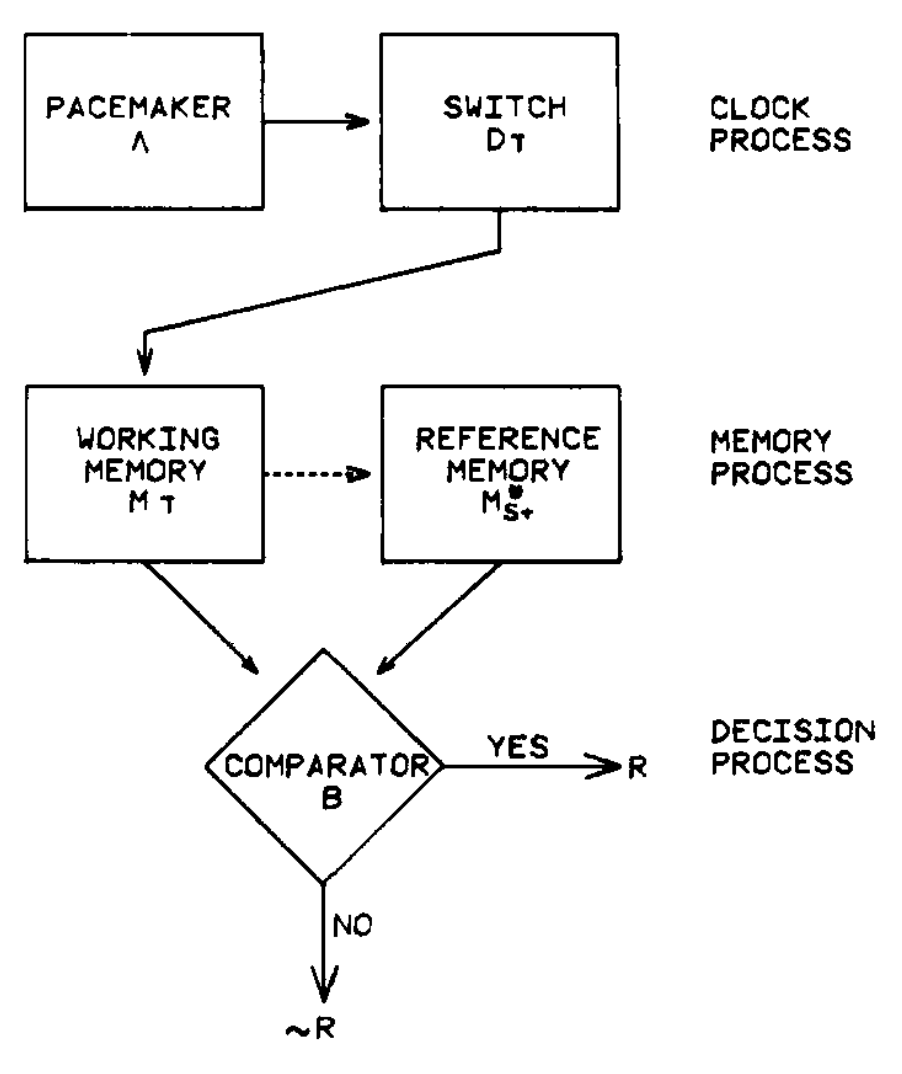
\includegraphics[width=5cm]{figures/SET_model_schema.png}
        \caption{Caption}
        \label{fig:set_schema}
    \end{figure}
    
    The SET model is by far the most popular timing model \cite{buhusi2005makes}, having retained attention from the community for more than 30 years. Even though it has limitations and fails to predict some results \cite{machado2009learning}, its simplicity seems to compensate for it. There are too many timing models to consider an exhaustive listing \cite{}, and we introduce those that best foster our examination across levels of analysis. 
    
    In terms of algorithm, it has been shown that Drift Diffusion Models (DDMs) are a more general framework that encompasses the SET, LET, and other common models \cite{balci2016decision}. DDMs are evidence-accumulation models, that compare the evidence among two alternatives in a noisy setting, and are optimal in the sense they can reach some predetermined accuracy in the least amount of time. They have the interesting uptick of being commonly used to study decision making, and thus frame timing in terms of decision. 
    
    At the level of implementation, the most discussed model is simply the ramping neuron \cite{}, where single neurons increase their activity up to a threshold that triggers the response. Single neuron models also feature time cells \cite{}, whose activity marks a point in time. Alternatively, there are a variety of state-dependent network models (SDNs) \cite{}, where time is represented in the collective activity of many neurons \cite{}. In the halfway, "synfire chains" model sequentially activated cell assemblies \cite{}. From these examples, state-dependent networks are the most general: all of the other models can be interpreted as SDNs \cite{}. However, instances of SDN proposed in the literature generally emphasize that trajectories in the phase space are intricate, in opposition to the elementary ones that could be represented by the simpler models \cite{}.

    There are many attempts to bridge the gap between Algorithm and Implementation, one of which is proposed by Simen et al. \cite{}. They build up from individual neurons to a DDM, by successive approximations, going through two steps of neural populations.
    
    \subsection{Intrinsic vs Dedicated}
        %Ler
        Among models of timing, there is an ongoing discussion on the intrinsicness of the processes involved in timing. While much of the discussion around time processing has 
        
% Converging data supports intrinsic models
\section{The taxonomy of timing}
\label{sub:taxonomy}

    The split between explicit and implicit memory was a breakthrough, providing a framework that enabled new kinds of questions \cite{paton2018neural}. % Change, explain
    
    % The scale of seconds has a name, but not clear boundaries. What constitutes interval timing may range from seconds to hours in some studies \cite{}, and from tens of milliseconds to seconds in others \cite{}. 
    
    The field of timing currently lacks a thorough taxonomy, grouping forms of timing that depend on similar circuits and mechanisms \cite{}, and distinguishing those that do not. Paton and Buonomano \cite{paton2018neural} proposed one such grouping, to be used as starting point in this endeavor. They considered the computational requirements of many tasks, and arrived at a three-dimensional account for them
    \begin{enumerate}
        \item \textit{Subsecond vc Suprasecond timing}. The most established dimension along with timing tasks vary, it is
        \item \textit{Motor vs Sensory timing}.
        \item \textit{Interval vs Pattern timing}.
    \end{enumerate}



\section{The anatomy of timing}
\label{sub:anatomy}
    
 % talvez caiba melhor na discussão
    The scale of time intervals is widely used as distinction between experiments \cite{van20168, buhusi2005makes, hardy2016neurocomputational}, and commonly considered sufficient to characterize timing tasks \cite{buhusi2005makes}. Accordingly, the scale of seconds to minutes is called \textit{Interval Timing}, and its characteristics are assessed through several tasks \cite{lloyd2012neural,astrand2014comparison,brea2016prospective,mello2015scalable,gouvea2015striatal,kopec2018controlling,gershman2014dopamine,tiganj2016sequential,narayanan2009delay,cho2010differential}. While neural structures necessary for good performance differ among Interval Timing tasks \cite{paton2018neural}, there may exist a single neural mechanism rendering the time representation \cite{gibbon1977scalar}, or still further a single region for Interval Timing common to all of them \cite{mello2015scalable}. Some common properties detected across tasks support this idea of a single mechanism underpinning all timing in the order of seconds \cite{buhusi2005makes, gibbon1977scalar}. The scalar property is the fact that errors in the time estimation are  proportional to the interval being estimated \cite{oprisan2014all}, and it is present as a feature of many models \cite{gibbon1977scalar, oprisan2014all}. The dependence on dopamine to its correct performance is also characteristic of Interval Timing tasks \cite{kim2017optogenetic, meck2012gene} -- excess of dopamine causes underestimation of intervals \cite{cheng2016clock, pine2010dopamine}, while lack of dopamine leads to their overestimation \cite{drew2003effects}. 
    
    Independently of how dedicated or intrinsic are time representations, an important role is traced to cortico-striatal circuits \cite{lusk2016utilizing, buhusi2005makes, meck2008cortico}, in special to the mPFC \cite{buhusi2018inactivation} and the Striatum \cite{mello2015scalable}.
        
    \subsection{Medial Pre-Frontal Cortex}
    % TODO anatomy
    % TODO connections
    % TODO functions
        The medial prefrontal cortex has been implicated in Timing in multiple tasks, such as Reaction Time \cite{narayanan2009delay}, Differential Reinforcement of Low rate \cite{cho2010differential} Temporal Bisection \cite{kim2009inactivation,tiganj2016sequential,kim2013neural}, and Peak Procedure \cite{buhusi2018inactivation}, by distinct methods such as lesions \cite{cho2010differential}, inactivation by muscimol \cite{buhusi2018inactivation, kim2009inactivation}, and optogenetic stimulation \cite{kim2017optogenetic}.
    % TODO timing
        
    \subsection{Striatum}
    % TODO anatomy
        The Striatum is a part of the basal ganglia, a series of nuclei that connect both to Cortex and Brainstem \cite{helie2015learning}. 
    % TODO connections
    % TODO functions
        Its traditional roles relate to procedural learning, and to the initiation and termination of movements \cite{helie2015learning}. Deficiencies in the basal ganglia might cause diseases like Parkinson's, in which patients' erratic movements and tremblings show deregulation of movements' bounds by lack of dopamine \cite{buhusi2005makes}. An intact Striatum is required for performing many Interval Timing tasks \cite{mello2015scalable,gouvea2015striatal,cho2010differential}, such that it is the centerpiece of many timing models \cite{mello2015scalable, buhusi2005makes}.
    % TODO timing
    
        While much has been done in the context of timing performance, the mechanisms through which the correct behavior develops during learning are much less studied \cite{van20168}.
